\chapter{Genética de populações e seleção natural}\label{ch:b2:population-genetics}

Em 1848, uma mariposa-salpicada preta foi capturada perto de Manchester;
em 1895, dezenove mariposas em cada vinte na cidade eram pretas e, em
1970, à medida que a fuligem desaparecia, a forma clara estava de volta.
As mariposas não mudaram: mudaram as proporções de dois \omterm{def:b2:meiosis-heredity:vocabulary}{alelos} numa
população de milhões, sob os olhos das aves, em algumas dezenas de
gerações. Darwin tinha visto que a seleção deve mudar as espécies, mas
não tinha como contá-la; a contagem é a \omterm{def:b2:population-genetics:frequencies}{genética de populações}, e ela é
a aritmética deste capítulo. Ela pergunta como as \omterm{def:b2:population-genetics:frequencies}{frequências alélicas}
se comportam quando nada age sobre elas e, depois, com que rapidez a
seleção, a \omterm{def:b2:genome-diversification:mutation}{mutação}, a migração, o acaso e a endogamia as deslocam --- e
termina com os caracteres que não são um gene, mas muitos, o que
constitui a maior parte do que a seleção de fato enxerga.

\section{O pool gênico em repouso}

\begin{definition}[População, pool gênico, frequências]\label{def:b2:population-genetics:frequencies}
\index{genética de populações}\index{pool gênico}\index{frequência alélica}
Uma \emph{população} é um grupo de indivíduos de uma espécie que se
cruzam entre si; seu \emph{pool gênico} é o conjunto de todos os seus
\omterm{def:b2:meiosis-heredity:vocabulary}{alelos}. Para um lócus com dois \omterm{def:b2:meiosis-heredity:vocabulary}{alelos} $A$ e $a$ numa população \omterm{def:b2:meiosis-heredity:meiosis}{diploide}
de $N$ indivíduos, as \emph{frequências alélicas} são $p = (2N_{AA} +
N_{Aa})/2N$ e $q = 1 - p$, e as \emph{frequências genotípicas} são as
frações de $AA$, $Aa$ e $aa$. A evolução, no sentido mais estrito, é uma
mudança das frequências alélicas entre gerações; a questão deste
capítulo é o que as muda e em que medida.
\end{definition}

\begin{theorem}[Hardy--Weinberg]\label{thm:b2:population-genetics:hw}
\index{lei de Hardy--Weinberg}
Numa população grande com cruzamentos ao acaso, sem seleção, \omterm{def:b2:genome-diversification:mutation}{mutação} ou
migração, as \omterm{def:b2:population-genetics:frequencies}{frequências alélicas} não mudam de uma geração para a
seguinte e, após uma única geração de cruzamentos ao acaso, as
frequências genotípicas são
\[
AA : p^{2}, \qquad Aa : 2pq, \qquad aa : q^{2},
\]
e assim permanecem. A dominância não faz um \omterm{def:b2:meiosis-heredity:vocabulary}{alelo} \omterm{def:b2:meiosis-heredity:vocabulary}{dominante} se
espalhar, e um \omterm{def:b2:meiosis-heredity:vocabulary}{alelo} \omterm{def:b2:meiosis-heredity:vocabulary}{recessivo} raro não se perde: ele se esconde nos
\omterm{def:b2:meiosis-heredity:vocabulary}{heterozigotos}, que superam os \omterm{def:b2:meiosis-heredity:vocabulary}{homozigotos} na razão de $2p/q$ para um ---
para $q = 0.01$, duzentos para um. A lei é a hipótese nula da \omterm{def:b2:population-genetics:frequencies}{genética
de populações}: um desvio dela numa população real, ou uma mudança de
$p$ entre gerações, é a assinatura de uma das forças descritas a
seguir.
\end{theorem}
\begin{proof}
O cruzamento ao acaso é a união ao acaso dos gametas: um gameta carrega
$A$ com probabilidade $p$ e $a$ com probabilidade $q$,
independentemente de seu parceiro, de modo que o zigoto é $AA$ com
probabilidade $p^{2}$, $Aa$ com $2pq$, $aa$ com $q^{2}$. A \omterm{def:b2:population-genetics:frequencies}{frequência
alélica} na geração seguinte é $p' = p^{2} + \tfrac12(2pq) = p(p + q) = p$: inalterada.
Como as frequências genotípicas dependem apenas de $p$, elas são as
mesmas em todas as gerações após a primeira.
\end{proof}

\begin{example}[Ler uma frequência]\label{ex:b2:population-genetics:cf}
A fibrose cística, recessiva, afeta uma criança europeia em 2500:
$q^{2} = 1/2500$, $q = 0.02$, e a frequência de portadores é $2pq
\approx 0.04$ --- uma pessoa em 25 carrega um \omterm{def:b2:meiosis-heredity:vocabulary}{alelo} que mata seus
\omterm{def:b2:meiosis-heredity:vocabulary}{homozigotos}, e \qty{98}{\%} das cópias do \omterm{def:b2:meiosis-heredity:vocabulary}{alelo} estão em portadores
saudáveis, onde a seleção não consegue enxergá-las. É por isso que um
\omterm{def:b2:meiosis-heredity:vocabulary}{recessivo} letal é eliminado tão lentamente, e por isso que os projetos
eugênicos de eliminar doenças recessivas esterilizando os afetados
nunca poderiam ter funcionado: a aritmética da próxima seção mostra quão
lentamente.
\end{example}

\section{Seleção}

\begin{definition}[Aptidão]\label{def:b2:population-genetics:fitness}
\index{aptidão}\index{coeficiente de seleção}
A \emph{aptidão} $w$ de um \omterm{def:b2:meiosis-heredity:vocabulary}{genótipo} é sua contribuição relativa em
descendentes para a geração seguinte --- a sobrevivência até a
reprodução vezes a fecundidade, em escala tal que o melhor \omterm{def:b2:meiosis-heredity:vocabulary}{genótipo}
tenha $w = 1$. O \emph{coeficiente de seleção} $s$ de um \omterm{def:b2:meiosis-heredity:vocabulary}{genótipo} é seu
déficit, $w = 1 - s$. A aptidão é uma propriedade de um \omterm{def:b2:meiosis-heredity:vocabulary}{genótipo} num
ambiente, e não de um \omterm{def:b2:meiosis-heredity:vocabulary}{alelo} em si: o \omterm{def:b2:meiosis-heredity:vocabulary}{alelo} da mariposa melânica tinha
$w > 1$ em relação ao claro sobre a \omterm{def:b2:plant-meristems:wood}{casca} coberta de fuligem e $w < 1$
sobre os liquens.
\end{definition}

\begin{theorem}[A seleção muda a frequência alélica]\label{thm:b2:population-genetics:selection}
\index{seleção natural!equação}
Com as \omterm{def:b2:population-genetics:fitness}{aptidões} genotípicas $w_{AA}$, $w_{Aa}$, $w_{aa}$, a \omterm{def:b2:population-genetics:fitness}{aptidão}
média é $\bar w = p^{2}w_{AA} + 2pq\,w_{Aa} + q^{2}w_{aa}$ e a
\omterm{def:b2:population-genetics:frequencies}{frequência alélica} na geração seguinte é
\[
p' = \frac{p^{2}w_{AA} + pq\,w_{Aa}}{\bar w}, \qquad
\Delta p = p' - p = \frac{pq\,\bigl[p(w_{AA} - w_{Aa}) + q(w_{Aa} - w_{aa})\bigr]}{\bar w}.
\]
Duas consequências. Primeiro, $\Delta p$ é proporcional a $pq$: a
seleção é mais rápida em frequências intermediárias e mais lenta quando
um \omterm{def:b2:meiosis-heredity:vocabulary}{alelo} é raro ou está quase fixado --- há pouca variação sobre a qual
agir. Segundo, contra um \omterm{def:b2:meiosis-heredity:vocabulary}{alelo} \omterm{def:b2:meiosis-heredity:vocabulary}{recessivo} ($w_{AA} = w_{Aa} = 1$, $w_{aa} =
1 - s$) a mudança é $\Delta q = -s\,pq^{2}/\bar w$, proporcional
a $q^{2}$: um \omterm{def:b2:meiosis-heredity:vocabulary}{recessivo} raro é quase invisível para a seleção, e reduzir
sua frequência à metade a partir de $0.01$ leva cerca de cem gerações,
mesmo quando seus \omterm{def:b2:meiosis-heredity:vocabulary}{homozigotos} são letais. Um \omterm{def:b2:meiosis-heredity:vocabulary}{alelo} \omterm{def:b2:meiosis-heredity:vocabulary}{dominante} favorável
se espalha depressa no início e depois estaciona no fim, pela mesma
razão.
\end{theorem}
\begin{proof}
Dos descendentes, uma fração $p^{2}w_{AA}/\bar w$ é $AA$ e
$2pq\,w_{Aa}/\bar w$ é $Aa$ (a frequência de cada \omterm{def:b2:meiosis-heredity:vocabulary}{genótipo} ponderada
por sua \omterm{def:b2:population-genetics:fitness}{aptidão} e renormalizada); os \omterm{def:b2:meiosis-heredity:vocabulary}{alelos} $A$ entre eles são todos os
do primeiro e metade dos do segundo, o que dá $p'$. Subtraindo $p =
p\bar w/\bar w$ e expandindo $\bar w$, obtém-se $\Delta p$. Para um
\omterm{def:b2:meiosis-heredity:vocabulary}{recessivo} letal ($s = 1$): $q' = q^{2}\cdot 0 + pq$ sobre $\bar w = 1 -
q^{2}$, de modo que $q' = q/(1 + q)$, logo $1/q' = 1/q + 1$ e, após $t$
gerações, $1/q_t = 1/q_0 + t$: passar de $q_0 = 0.01$ a $0.005$ leva
$t = 100$.
\end{proof}

\begin{omfigure}
\begin{tikzpicture}
\begin{axis}[
  width=0.8\linewidth, height=6cm,
  axis x line=bottom, axis y line=left,
  xmin=0, xmax=150, ymin=0, ymax=1.05,
  xlabel={gerações}, ylabel={frequência do alelo favorecido},
  xlabel style={font=\small, at={(axis description cs:0.5,-0.11)}, anchor=north},
  ylabel style={font=\small},
  tick label style={font=\small}, xtick={0,50,100,150}, ytick={0,0.5,1},
  legend style={font=\scriptsize, at={(0.97,0.35)}, anchor=east, draw=none},
  clip=false,
]
\addplot[very thick, omDef] table[x=t, y=dom] {
t dom
0 0.01
10 0.02
20 0.04
30 0.075
40 0.14
50 0.24
60 0.38
70 0.53
80 0.66
90 0.76
100 0.83
110 0.88
120 0.91
130 0.93
140 0.945
150 0.955
};
\addlegendentry{alelo favorecido dominante, $s = 0.1$}
\addplot[very thick, omThm] table[x=t, y=rec] {
t rec
0 0.01
10 0.0101
20 0.0102
30 0.0104
40 0.0106
50 0.0108
60 0.011
70 0.0113
80 0.0116
90 0.012
100 0.0124
110 0.0128
120 0.0133
130 0.0138
140 0.0144
150 0.015
};
\addlegendentry{alelo favorecido recessivo, $s = 0.1$}
\end{axis}
\end{tikzpicture}

{\small A seleção em ação com uma vantagem de \qty{10}{\%}. Um \omterm{def:b2:meiosis-heredity:vocabulary}{alelo}
\omterm{def:b2:meiosis-heredity:vocabulary}{dominante} favorecido sobe de \qty{1}{\%} até a maioria em setenta
gerações e depois desacelera, pois seu raro rival \omterm{def:b2:meiosis-heredity:vocabulary}{recessivo} se esconde
nos \omterm{def:b2:meiosis-heredity:vocabulary}{heterozigotos}; um \omterm{def:b2:meiosis-heredity:vocabulary}{alelo} \omterm{def:b2:meiosis-heredity:vocabulary}{recessivo} favorecido a \qty{1}{\%} quase não
se move no mesmo tempo, já que quase nunca fica exposto.}
\end{omfigure}

\begin{proposition}[Tipos de seleção]\label{prop:b2:population-genetics:kinds}
\index{seleção direcional}\index{seleção estabilizadora}\index{seleção balanceadora}\index{vantagem do heterozigoto}
A seleção \emph{direcional} favorece um extremo e leva um \omterm{def:b2:meiosis-heredity:vocabulary}{alelo} à
fixação (a mariposa melânica num bosque coberto de fuligem; a
resistência aos antibióticos; o tamanho do bico de um tentilhão numa
seca). A seleção \emph{estabilizadora} favorece o meio e elimina os
extremos (o peso ao nascer humano: os bebês que morrem são os menores e
os maiores); ela mantém uma população onde está e é o tipo mais comum.
A seleção \emph{disruptiva} favorece os dois extremos contra o meio e
pode dividir uma população (\cref{ch:b2:speciation}). A seleção
\emph{balanceadora} mantém dois \omterm{def:b2:meiosis-heredity:vocabulary}{alelos} na população indefinidamente:
pela \emph{\omterm{prop:b2:population-genetics:kinds}{vantagem do heterozigoto}}, quando $Aa$ tem \omterm{def:b2:population-genetics:fitness}{aptidão} maior que
qualquer dos \omterm{def:b2:meiosis-heredity:vocabulary}{homozigotos} --- com
$w_{AA} = 1 - s$, $w_{aa} = 1 - t$, $w_{Aa} = 1$, a frequência
se estabiliza em $\hat p = t/(s + t)$ --- ou pela seleção \emph{dependente
da frequência}, quando um \omterm{def:b2:meiosis-heredity:vocabulary}{genótipo} tem \omterm{def:b2:population-genetics:fitness}{aptidão} maior quanto mais raro é
(os \omterm{def:b2:meiosis-heredity:vocabulary}{alelos} $S$ raros do \cref{ch:b2:angiosperm-reproduction}, as presas
que um predador ainda não aprendeu a reconhecer, os dois lados da boca
de um peixe comedor de escamas).
\end{proposition}
\begin{proof}[Evidências]
A hemoglobina falciforme mata a maioria dos \omterm{def:b2:meiosis-heredity:vocabulary}{homozigotos} antes que se
reproduzam, e no entanto o \omterm{def:b2:meiosis-heredity:vocabulary}{alelo} está entre \qty{10}{\%} e \qty{20}{\%}
em toda a África malárica. Allison (1954) mostrou que as crianças
heterozigotas tinham infecções maláricas muito menos numerosas e mais
brandas que qualquer dos \omterm{def:b2:meiosis-heredity:vocabulary}{homozigotos}, e a frequência do \omterm{def:b2:meiosis-heredity:vocabulary}{alelo} acompanha
a distribuição histórica da malária por falciparum; nas populações de
ascendência africana que vivem onde não há malária, a frequência vem
caindo desde então. Com $t \approx 0.8$ para o \omterm{def:b2:meiosis-heredity:vocabulary}{homozigoto} falciforme
e $s \approx 0.1$ para o \omterm{def:b2:meiosis-heredity:vocabulary}{homozigoto} normal numa região malárica,
$\hat q = s/(s + t) \approx 0.11$ --- o que se observa.
\end{proof}

\section{Mutação, migração e o equilíbrio}

\begin{theorem}[Equilíbrio mutação--seleção]\label{thm:b2:population-genetics:balance}
\index{equilíbrio mutação--seleção}\index{carga genética}
Um \omterm{def:b2:meiosis-heredity:vocabulary}{alelo} deletério é alimentado pela \omterm{def:b2:genome-diversification:mutation}{mutação} à taxa $\mu$ por gameta por
geração e removido pela seleção. No equilíbrio, as duas se compensam:
para um \omterm{def:b2:meiosis-heredity:vocabulary}{alelo} \omterm{def:b2:meiosis-heredity:vocabulary}{recessivo} com desvantagem homozigota $s$,
\[
\hat q = \sqrt{\mu/s}\,;
\]
para um \omterm{def:b2:meiosis-heredity:vocabulary}{alelo} \omterm{def:b2:meiosis-heredity:vocabulary}{dominante} (ou parcialmente \omterm{def:b2:meiosis-heredity:vocabulary}{dominante}) com desvantagem
heterozigota $hs$, $\hat q = \mu/hs$. A frequência de equilíbrio de um
\omterm{def:b2:meiosis-heredity:vocabulary}{recessivo} é, portanto, grande mesmo para um letal: com $\mu = 10^{-5}$ e
$s = 1$, $\hat q = 3\times 10^{-3}$, e \qty{0.6}{\%} da população
o carrega. Toda população carrega essa \emph{\omterm{thm:b2:population-genetics:balance}{carga genética}} em milhares
de lócus, a maior parte recessiva e oculta, e o equilíbrio do argumento
da catraca do \cref{ch:b2:asexual-reproduction}
--- uma fração $e^{-U/s}$ de indivíduos livres de \omterm{def:b2:genome-diversification:mutation}{mutações}
deletérias --- é o mesmo equilíbrio somado sobre o genoma.
\end{theorem}
\begin{proof}
A cada geração, a \omterm{def:b2:genome-diversification:mutation}{mutação} acrescenta $\mu p \approx \mu$ a $q$ e a
seleção remove $s\,pq^{2}/\bar w \approx sq^{2}$ (para $q$ pequeno);
fazer $\mu = s\hat q^{2}$ dá o resultado \omterm{def:b2:meiosis-heredity:vocabulary}{recessivo}. Para um \omterm{def:b2:meiosis-heredity:vocabulary}{alelo}
\omterm{def:b2:meiosis-heredity:vocabulary}{dominante}, a seleção remove $hs\,q$ por geração (cada cópia fica exposta
num \omterm{def:b2:meiosis-heredity:vocabulary}{heterozigoto}), e $\mu = hs\hat q$.
\end{proof}

\begin{proposition}[Migração e a regra de um migrante]\label{prop:b2:population-genetics:migration}
\index{fluxo gênico}\index{migração (genética)}
Se uma fração $m$ de uma população é, a cada geração, formada por
imigrantes de uma população com \omterm{def:b2:population-genetics:frequencies}{frequência alélica} $p_{m}$, a frequência
se desloca em direção a $p_{m}$ em $\Delta p = m(p_{m} - p)$: a diferença
entre as duas populações decai como $(1 - m)^{t}$. O \emph{\omterm{prop:b2:population-genetics:migration}{fluxo
gênico}} homogeneíza; ele desfaz a \omterm{def:b2:plant-plasticity:plasticity}{adaptação} local, a menos que a seleção
seja mais forte que $m$, e é a força que mantém uma espécie como uma só
espécie. Inversamente, populações que não trocam migrantes divergem por
deriva e por suas \omterm{def:b2:genome-diversification:mutation}{mutações} próprias, e um único migrante por geração ---
qualquer que seja o tamanho da população --- basta para impedir que elas
fixem \omterm{def:b2:meiosis-heredity:vocabulary}{alelos} diferentes por deriva.
\end{proposition}

\section{O acaso: a deriva genética}

\begin{theorem}[Deriva genética]\label{thm:b2:population-genetics:drift}
\index{deriva genética}\index{tamanho efetivo da população}\index{fixação}
Numa população de $N$ indivíduos \omterm{def:b2:meiosis-heredity:meiosis}{diploides}, a \omterm{def:b2:population-genetics:frequencies}{frequência alélica} de cada
geração é uma amostra aleatória de $2N$ gametas da anterior, de modo que
$p$ vagueia ao acaso com uma variância de
$p(1 - p)/2N$ por geração. A \emph{heterozigosidade} $H = 2pq$
decai em média por um fator $(1 - 1/2N)$ a cada geração,
\[
H_t = H_0\left(1 - \frac{1}{2N}\right)^{t} \approx H_0\,e^{-t/2N},
\]
e todo \omterm{def:b2:meiosis-heredity:vocabulary}{alelo} acaba perdido ou \emph{fixado}, com probabilidade igual à
sua frequência atual: uma nova \omterm{def:b2:genome-diversification:mutation}{mutação} neutra, com frequência $1/2N$, é
fixada com probabilidade $1/2N$ e, se o for, leva cerca de $4N$ gerações
para isso. A deriva é desprezível numa população de milhões e dominante
numa de dezenas: um \emph{gargalo} ou um evento \emph{fundador} --- alguns
colonos numa ilha, uma espécie reduzida a uma centena pela caça ---
perde \omterm{def:b2:meiosis-heredity:vocabulary}{alelos} por acaso em uma geração e deixa uma população uniforme,
empobrecida e cheia de \omterm{def:b2:meiosis-heredity:vocabulary}{homozigotos}. O $N$ que importa é o tamanho
\emph{efetivo}, o número de indivíduos que de fato se reproduzem,
geralmente muito menor que o do recenseamento.
\end{theorem}
\begin{proof}
As $2N$ cópias gênicas da geração seguinte são sorteadas com reposição
de um conjunto em que $A$ tem frequência $p$: o número de cópias de $A$
é binomial, com média $2Np$ e variância $2Np(1 - p)$, de modo que $p'$
tem média $p$ e variância $p(1 - p)/2N$. Duas cópias sorteadas ao acaso
na geração seguinte provêm da mesma cópia parental com probabilidade
$1/2N$ e são então idênticas, de modo que a chance de duas cópias
diferirem (a heterozigosidade) é multiplicada por $1 - 1/2N$ a cada
geração. Probabilidade de fixação: a frequência de um \omterm{def:b2:meiosis-heredity:vocabulary}{alelo} neutro é uma
martingale --- seu valor esperado nunca muda --- e termina em 0 ou 1, de
modo que a probabilidade de terminar em 1 é igual a seu valor inicial.
\end{proof}

\begin{omfigure}
\begin{tikzpicture}
\begin{axis}[
  width=0.82\linewidth, height=6cm,
  axis x line=bottom, axis y line=left,
  xmin=0, xmax=60, ymin=0, ymax=1.05,
  xlabel={gerações}, ylabel={frequência alélica $p$},
  xlabel style={font=\small, at={(axis description cs:0.5,-0.11)}, anchor=north},
  ylabel style={font=\small},
  tick label style={font=\small}, xtick={0,20,40,60}, ytick={0,0.5,1},
  legend style={font=\scriptsize, at={(0.5,-0.25)}, anchor=north, draw=none, legend columns=2},
  clip=false,
]
\addplot[thick, omThm] coordinates {(0,0.5) (2,0.55) (4,0.62) (6,0.58) (8,0.7) (10,0.8) (12,0.75) (14,0.85) (16,0.92) (18,0.88) (20,0.95) (22,1) (60,1)};
\addlegendentry{$N = 10$}
\addplot[thick, omThm!60] coordinates {(0,0.5) (2,0.42) (4,0.35) (6,0.4) (8,0.3) (10,0.2) (12,0.25) (14,0.15) (16,0.1) (18,0.05) (20,0.08) (22,0.02) (24,0) (60,0)};
\addplot[thick, omDef] coordinates {(0,0.5) (5,0.52) (10,0.49) (15,0.53) (20,0.56) (25,0.54) (30,0.58) (35,0.55) (40,0.57) (45,0.6) (50,0.58) (55,0.61) (60,0.6)};
\addlegendentry{$N = 1000$}
\addplot[thick, omDef!60] coordinates {(0,0.5) (5,0.48) (10,0.5) (15,0.47) (20,0.45) (25,0.46) (30,0.44) (35,0.45) (40,0.43) (45,0.44) (50,0.42) (55,0.43) (60,0.42)};
\end{axis}
\end{tikzpicture}

{\small Deriva. Duas populações de dez indivíduos que partem de
$p = 0.5$ fixam \omterm{def:b2:meiosis-heredity:vocabulary}{alelos} opostos em vinte e cinco gerações; duas de mil
vagueiam alguns por cento em sessenta.}
\end{omfigure}

\begin{proposition}[Endogamia]\label{prop:b2:population-genetics:inbreeding}
\index{endogamia}\index{coeficiente de endogamia}\index{depressão por endogamia}
O cruzamento entre parentes não muda as \omterm{def:b2:population-genetics:frequencies}{frequências alélicas}, mas
aumenta a proporção de \omterm{def:b2:meiosis-heredity:vocabulary}{homozigotos}: o \emph{\omterm{prop:b2:population-genetics:inbreeding}{coeficiente de endogamia}}
$F$ de um indivíduo é a probabilidade de que seus dois \omterm{def:b2:meiosis-heredity:vocabulary}{alelos} num lócus
sejam idênticos por descendência, e as frequências genotípicas passam a
ser $p^{2} + Fpq$, $2pq(1 - F)$, $q^{2} + Fpq$. Para os filhos de primos
em primeiro grau, $F = 1/16$; de irmãos, $1/4$; de autofecundação,
$1/2$. Como os \omterm{def:b2:meiosis-heredity:vocabulary}{alelos} \omterm{def:b2:meiosis-heredity:vocabulary}{recessivos} da \omterm{thm:b2:population-genetics:balance}{carga genética} ficam expostos nos
\omterm{def:b2:meiosis-heredity:vocabulary}{homozigotos} adicionais, os descendentes endogâmicos sofrem
\emph{\omterm{prop:b2:population-genetics:inbreeding}{depressão por endogamia}}: um \omterm{def:b2:meiosis-heredity:vocabulary}{recessivo} letal a $q = 0.01$
aparece em $q^{2} = 10^{-4}$ dos descendentes de cruzamentos ao acaso, mas em
$q^{2} + Fpq = 7\times 10^{-4}$ dos filhos de primos, sete vezes mais;
somados sobre milhares de lócus, os filhos de primos têm cerca do dobro
da mortalidade infantil dos demais, e uma população pequena que se
cruza entre parentes por gerações perde fertilidade e vigor --- a
situação do guepardo, da pantera-da-flórida e das casas reais da Europa.
\end{proposition}

\section{Muitos genes: caracteres quantitativos}

\begin{theorem}[Herdabilidade e resposta à seleção]\label{thm:b2:population-genetics:heritability}
\index{herdabilidade}\index{genética quantitativa}\index{equação do melhorista}
Um caráter como a altura, o rendimento ou a profundidade do bico é
determinado por muitos genes de pequeno efeito e pelo ambiente, e varia
de modo contínuo. Sua variância numa população se divide numa parte
\emph{genética} $V_G$ e numa parte \emph{ambiental} $V_E$, e
a \emph{herdabilidade} $h^{2} = V_A/V_P$ é a fração da variância
fenotípica devida aos efeitos aditivos dos genes (a parte que é
transmitida). Se os pais da geração seguinte são selecionados com uma
média que excede a da população em $S$ (o \emph{diferencial de
seleção}), seus descendentes a excedem em
\[
R = h^{2}\,S
\]
--- a \emph{\omterm{thm:b2:population-genetics:heritability}{equação do melhorista}}. Ela resume todo o melhoramento animal e
vegetal numa linha: uma herdabilidade de $0.5$ e pais um desvio-padrão
acima da média dão descendentes meio desvio-padrão acima dela, e o ganho
se acumula geração após geração. A herdabilidade é uma propriedade de
uma população num ambiente, e não de um caráter: ela não diz nada sobre
se um traço é fixo, e um traço com $h^{2} = 0.8$ numa população pode
ter $h^{2} = 0$ em outra, na qual todos os indivíduos têm o mesmo
\omterm{def:b2:meiosis-heredity:vocabulary}{genótipo}.
\end{theorem}
\begin{proof}
O \omterm{def:b2:meiosis-heredity:vocabulary}{fenótipo} esperado dos descendentes regride sobre o dos pais médios
com inclinação $h^{2}$ (a covariância genética aditiva entre parentes
dividida pela variância fenotípica), de modo que um desvio parental $S$
dá um desvio dos descendentes $h^{2}S$. Na prática, $h^{2}$ é medido a
partir dessa regressão, ou da semelhança entre gêmeos e irmãos, ou da
própria resposta.
\end{proof}
\begin{proof}[Evidências]
O experimento do milho de Illinois, iniciado em 1896, selecionou todos
os anos as espigas com o maior e o menor teor de óleo: após cem gerações,
a linhagem alta tinha subido de \qty{5}{\%} para \qty{20}{\%} de óleo e
a baixa caído para menos de \qty{1}{\%}, ambas ainda respondendo --- a
variação de muitos genes não se esgota em um século de seleção. Nas
Galápagos, os Grant mediram todos os tentilhões de uma ilha durante a
seca de 1977: os sobreviventes tinham bicos \qty{4}{\%} mais profundos
que os mortos, o caráter tinha $h^{2}
\approx 0.7$, e os filhotes do ano seguinte tinham bicos
\qty{3}{\%} mais profundos que os da geração anterior --- a seleção
observada, medida e com sua resposta prevista pela equação
acima.
\end{proof}

\begin{omfigure}
\begin{tikzpicture}
\begin{axis}[
  width=0.78\linewidth, height=5.6cm,
  axis x line=bottom, axis y line=left,
  xmin=6, xmax=14, ymin=0, ymax=0.32,
  xlabel={profundidade do bico (mm)}, ylabel={frequência},
  xlabel style={font=\small, at={(axis description cs:0.5,-0.12)}, anchor=north},
  ylabel style={font=\small},
  tick label style={font=\small}, xtick={7,9,11,13}, ytick=\empty,
  legend style={font=\scriptsize, at={(0.5,-0.28)}, anchor=north, draw=none, legend columns=3},
  clip=false,
]
\addplot[very thick, omDef, domain=6:14, samples=100] {0.3*exp(-((x-9.4)^2)/(2*0.9))};
\addlegendentry{antes da seca, média 9.4}
\addplot[very thick, omThm, domain=6:14, samples=100] {0.28*exp(-((x-9.9)^2)/(2*0.8))};
\addlegendentry{sobreviventes, média 9.9}
\addplot[very thick, omProp, dashed, domain=6:14, samples=100] {0.3*exp(-((x-9.75)^2)/(2*0.9))};
\addlegendentry{geração seguinte, média 9.75}
\draw[<->] (axis cs:9.4,0.02) -- (axis cs:9.9,0.02); \node[font=\scriptsize, anchor=south] at (axis cs:9.65,0.025) {$S$};
\end{axis}
\end{tikzpicture}

{\small A \omterm{thm:b2:population-genetics:heritability}{equação do melhorista} numa população de tentilhões. A seca
deixou sobreviventes com um bico médio $S = \qty{0.5}{mm}$ mais
profundo; com $h^{2} = 0.7$, seus descendentes foram $R = \qty{0.35}{mm}$
mais profundos que a geração anterior.}
\end{omfigure}

\begin{example}[A aritmética da mariposa]\label{ex:b2:population-genetics:moth}
O \omterm{def:b2:meiosis-heredity:vocabulary}{alelo} melânico da mariposa-salpicada é \omterm{def:b2:meiosis-heredity:vocabulary}{dominante}. Passar de uma
frequência de cerca de $10^{-3}$ em 1848 a \qty{90}{\%} das mariposas
(uma frequência perto de $0.7$) em 1895 são cinquenta gerações; a
equação de seleção o reproduz com $s$ entre $0.2$ e $0.3$ contra a forma
clara --- e os experimentos de soltura de Kettlewell nos anos 1950, em
que as aves pegavam mariposas claras nos troncos com fuligem e escuras
nos troncos limpos mais ou menos nessa razão, mediram o coeficiente
diretamente. O retorno após as leis do ar limpo, de \qty{90}{\%} de
melânicas em 1960 a menos de \qty{10}{\%} em 2000, ocorreu na mesma
velocidade no sentido oposto. O episódio inteiro --- uma população
grande, um \omterm{def:b2:meiosis-heredity:vocabulary}{alelo} \omterm{def:b2:meiosis-heredity:vocabulary}{dominante}, um agente seletivo forte e reversível --- é
a \omterm{def:b2:population-genetics:frequencies}{genética de populações} acontecendo em público.
\end{example}

\begin{omfigure}
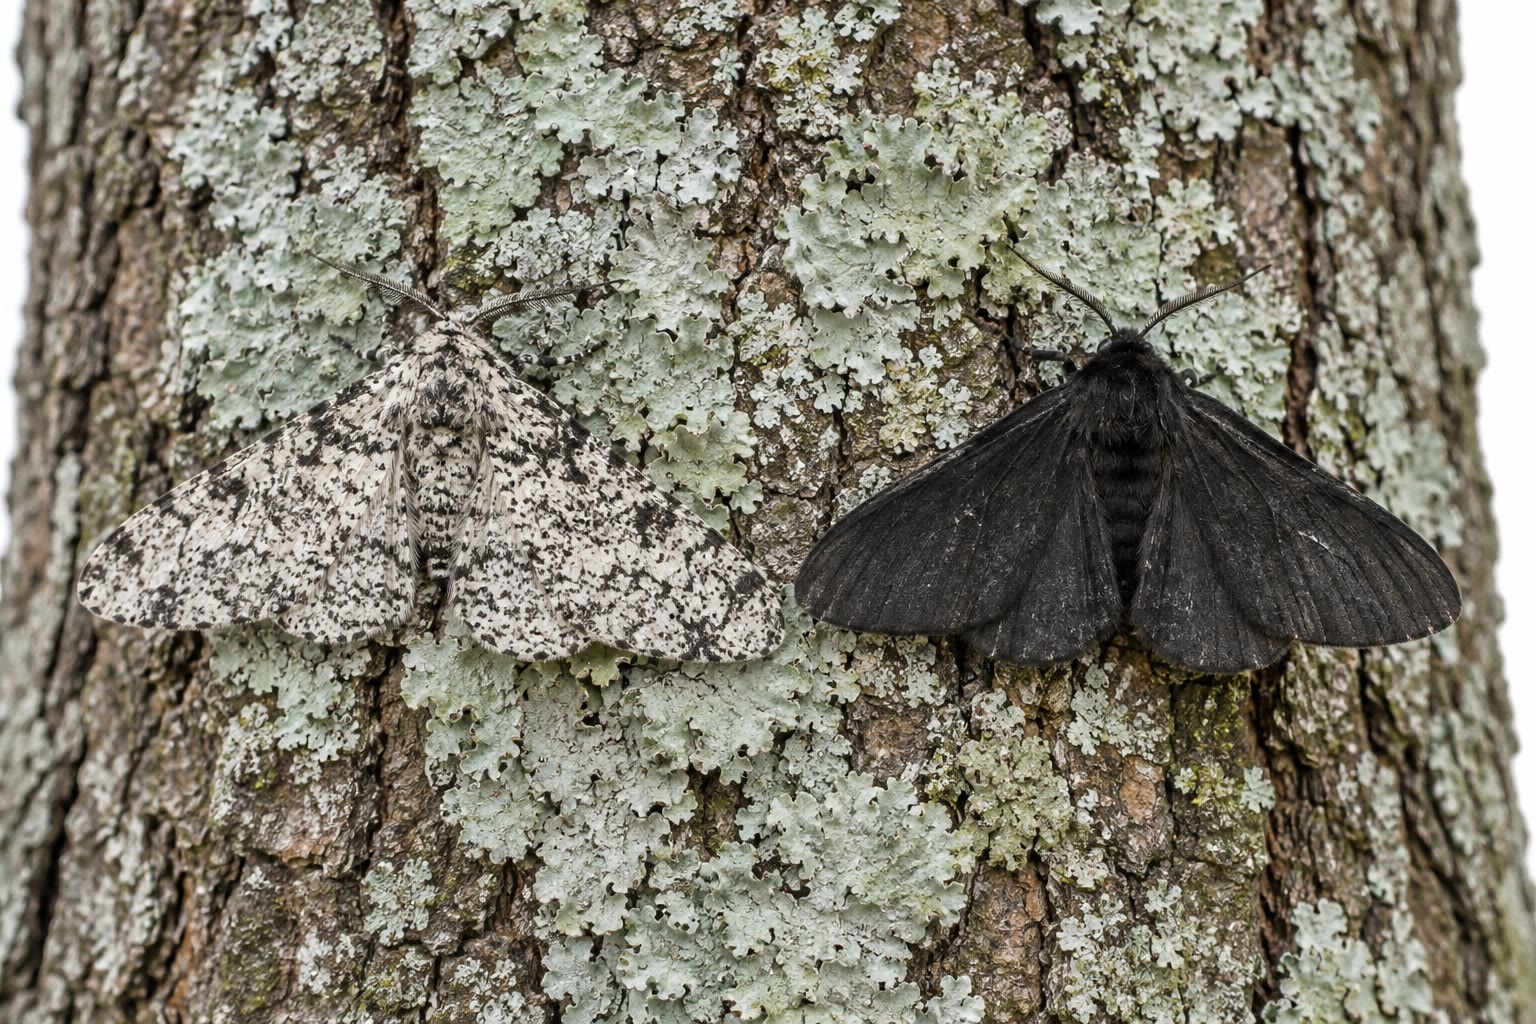
\includegraphics[width=0.46\linewidth]{images/book4/ai/b4-22-peppered-moths.jpg}\hspace{0.04\linewidth}
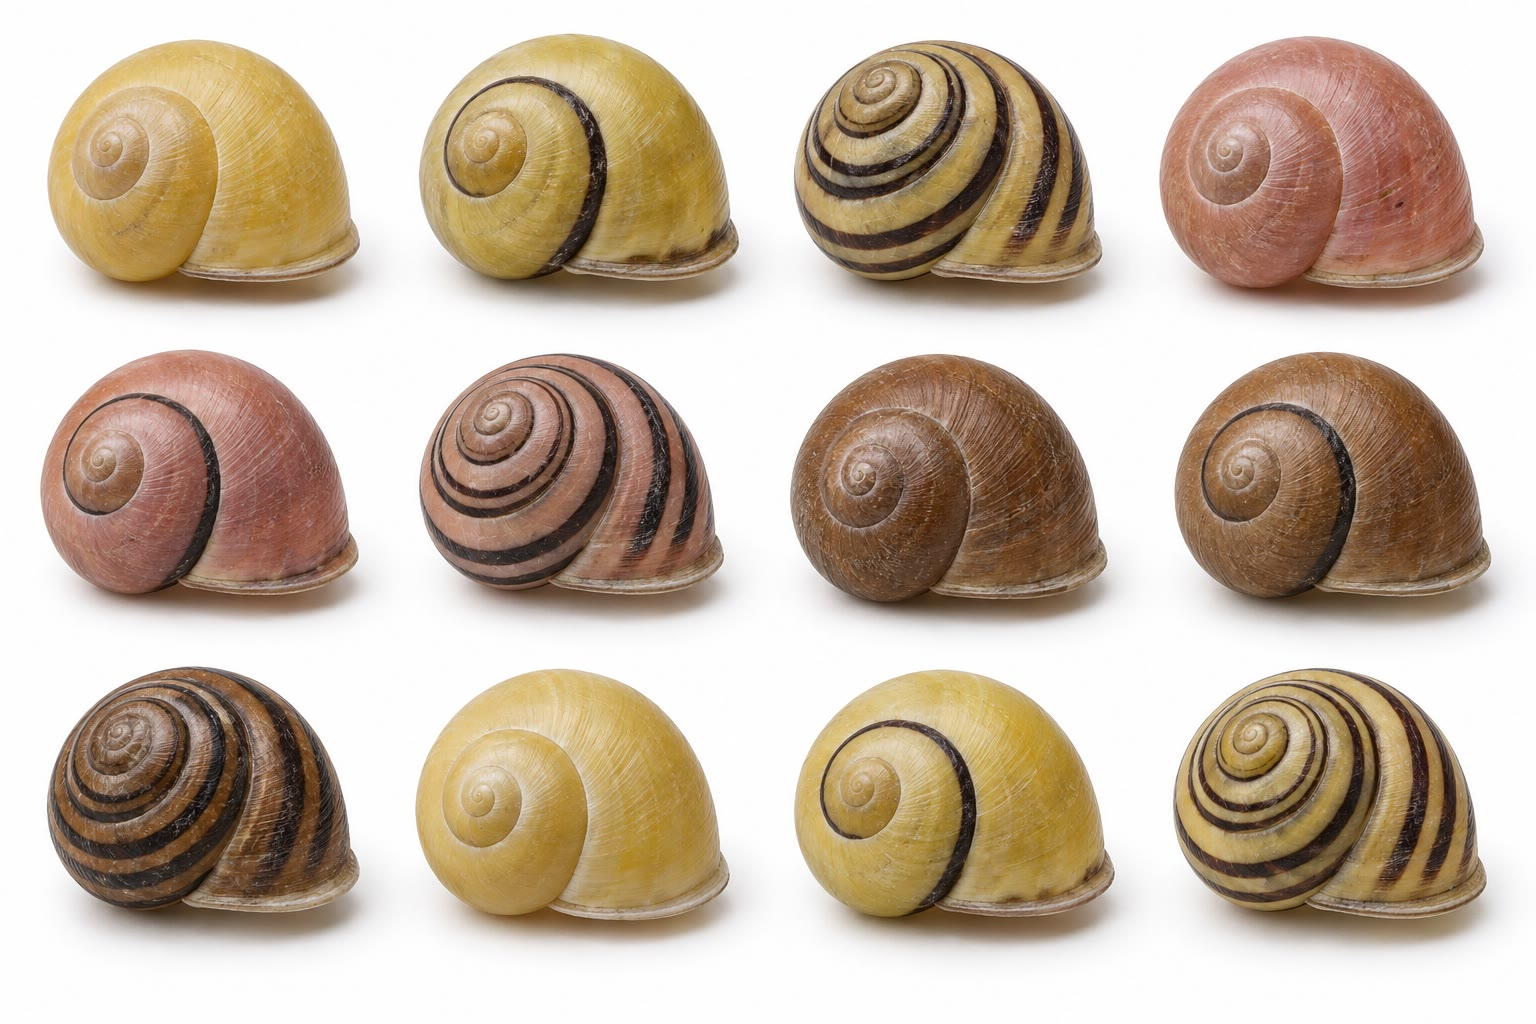
\includegraphics[width=0.46\linewidth]{images/book4/ai/b4-22-banded-snails.jpg}

{\small À esquerda: as duas formas da mariposa-salpicada sobre liquens
--- qual delas uma ave encontra depende da \omterm{def:b2:plant-meristems:wood}{casca}. À direita: o
polimorfismo da concha do caracol-dos-bosques, cores e faixas mantidas
em toda população por predadores que aprendem a forma comum.}
\end{omfigure}

\section{Exercícios}

\begin{exercise}[$\star$]\label{exo:b2:population-genetics:1}
Numa amostra de 1000 pessoas, 640 são $MM$, 320 $MN$ e 40 $NN$.
Calcule as \omterm{def:b2:population-genetics:frequencies}{frequências alélicas} e as proporções esperadas de
Hardy--Weinberg. A população está em equilíbrio?
\end{exercise}

\begin{exercise}[$\star$]\label{exo:b2:population-genetics:2}
O albinismo é \omterm{def:b2:meiosis-heredity:vocabulary}{recessivo} e afeta uma pessoa em \num{20000}.
Calcule a \omterm{def:b2:population-genetics:frequencies}{frequência alélica} e a frequência de portadores.
\end{exercise}

\begin{exercise}[$\star$]\label{exo:b2:population-genetics:3}
Defina \omterm{def:b2:population-genetics:fitness}{aptidão}, \omterm{def:b2:population-genetics:fitness}{coeficiente de seleção} e herdabilidade, e cite as
cinco forças que mudam as \omterm{def:b2:population-genetics:frequencies}{frequências alélicas}.
\end{exercise}

\begin{exercise}[$\star$]\label{exo:b2:population-genetics:4}
Dê um exemplo de \omterm{prop:b2:population-genetics:kinds}{seleção direcional}, um de estabilizadora e um de
balanceadora, com o agente de seleção em cada caso.
\end{exercise}

\begin{exercise}[$\star\star$]\label{exo:b2:population-genetics:5}
Um \omterm{def:b2:meiosis-heredity:vocabulary}{alelo} \omterm{def:b2:meiosis-heredity:vocabulary}{recessivo} letal tem frequência $0.02$. Quantas gerações são
necessárias para reduzi-la à metade? E para chegar a $0.001$? O que isso
diz sobre o efeito de impedir que os indivíduos afetados se reproduzam?
\end{exercise}

\begin{exercise}[$\star\star$]\label{exo:b2:population-genetics:6}
Com $w_{AA} = 1$, $w_{Aa} = 1$, $w_{aa} = 0.8$ e $p = 0.3$, calcule
$\bar w$, $p'$ e $\Delta p$. Repita para $p = 0.9$. Por que a
segunda mudança é tão menor?
\end{exercise}

\begin{exercise}[$\star\star$]\label{exo:b2:population-genetics:7}
O \omterm{def:b2:meiosis-heredity:vocabulary}{homozigoto} falciforme tem $w = 0.2$ e o \omterm{def:b2:meiosis-heredity:vocabulary}{homozigoto} normal
$w = 0.88$ numa região malárica, e os \omterm{def:b2:meiosis-heredity:vocabulary}{heterozigotos} $w = 1$. Calcule a
frequência de equilíbrio do \omterm{def:b2:meiosis-heredity:vocabulary}{alelo} falciforme e a fração de crianças que
nascem com a doença no equilíbrio.
\end{exercise}

\begin{exercise}[$\star\star$]\label{exo:b2:population-genetics:8}
Um letal \omterm{def:b2:meiosis-heredity:vocabulary}{recessivo} surge por \omterm{def:b2:genome-diversification:mutation}{mutação} a $\mu = \qty{2e-5}{}$ por
gameta. Calcule sua frequência de equilíbrio e a fração de nascimentos
afetados. Um letal \omterm{def:b2:meiosis-heredity:vocabulary}{dominante} (antes da reprodução) à mesma taxa: que
fração dos nascimentos?
\end{exercise}

\begin{exercise}[$\star\star$]\label{exo:b2:population-genetics:9}
Uma população de 50 indivíduos reprodutores começa com $H = 0.5$.
Calcule sua heterozigosidade após 10, 50 e 200 gerações. Qual deve ser
o tamanho de uma população para conservar \qty{90}{\%} de sua
heterozigosidade ao longo de 100 gerações?
\end{exercise}

\begin{exercise}[$\star\star\star$]\label{exo:b2:population-genetics:10}
Uma ilha é colonizada por 10 aves vindas de uma população continental
na qual um \omterm{def:b2:meiosis-heredity:vocabulary}{alelo} tem frequência $0.1$. Calcule a probabilidade de que o
\omterm{def:b2:meiosis-heredity:vocabulary}{alelo} esteja ausente dos fundadores e a probabilidade de que ele acabe
fixado na ilha se estiver presente em uma cópia. Compare com o
continente.
\end{exercise}

\begin{exercise}[$\star\star\star$]\label{exo:b2:population-genetics:11}
A produção de leite tem $h^{2} = 0.3$ e um desvio-padrão de
\qty{1000}{L}. Um criador mantém os \qty{20}{\%} melhores das vacas como
mães (sua média está $1.4$ desvio-padrão acima da do rebanho).
Calcule a resposta por geração. Se os touros forem escolhidos entre o
\qty{1}{\%} melhor (média $2.7$ desvios-padrão acima), qual é a
resposta? Por que a resposta desacelera após muitas gerações?
\end{exercise}

\begin{exercise}[$\star\star\star$]\label{exo:b2:population-genetics:12}
``A seleção é cega para o que não consegue ver.'' Discuta, com o
\omterm{def:b2:meiosis-heredity:vocabulary}{alelo} \omterm{def:b2:meiosis-heredity:vocabulary}{recessivo} nos \omterm{def:b2:meiosis-heredity:vocabulary}{heterozigotos}, a \omterm{def:b2:genome-diversification:mutation}{mutação} neutra e o caráter de
herdabilidade nula, sobre o que a seleção pode e não pode
agir.
\end{exercise}

\section{Problema: A mariposa, a ilha e o rebanho}

\begin{problem}[{Problema de fim de semana --- a ascensão da
mariposa-salpicada calculada a partir da equação de seleção, a deriva e
a endogamia de uma população fundadora acompanhadas, um equilíbrio
mutação--seleção estabelecido e um programa de melhoramento previsto,
terminando com o coeficiente de seleção da mariposa, a heterozigosidade
da ilha e o ganho do rebanho}]
\label{pb:b2:population-genetics:1}
Mariposa-salpicada: \omterm{def:b2:meiosis-heredity:vocabulary}{alelo} melânico $M$ \omterm{def:b2:meiosis-heredity:vocabulary}{dominante}, frequência $p_0 = 0.001$
em 1848; \qty{90}{\%} das mariposas melânicas 50 gerações depois; suponha
$w_{MM} = w_{Mm} = 1$ e $w_{mm} = 1 - s$. Ilha: fundada por 12
aves vindas de um continente onde $H = 0.4$ e um \omterm{def:b2:meiosis-heredity:vocabulary}{alelo} \omterm{def:b2:meiosis-heredity:vocabulary}{recessivo}
deletério tem $q = 0.05$; a ilha abriga daí em diante 40 aves
reprodutoras. \omterm{def:b2:genome-diversification:mutation}{Mutação}: $\mu = \qty{1e-5}{}$. Rebanho: $h^{2} = 0.4$,
desvio-padrão de \qty{800}{L}.

\medskip
\noindent\textbf{Parte I --- A mariposa.}
\begin{enumerate}
  \item Em 1848, que fração das mariposas era melânica, e que fração
        dos \omterm{def:b2:meiosis-heredity:vocabulary}{alelos} $M$ estava em \omterm{def:b2:meiosis-heredity:vocabulary}{heterozigotos}?
  \item Mostre que, com $M$ \omterm{def:b2:meiosis-heredity:vocabulary}{dominante}, a frequência do \omterm{def:b2:meiosis-heredity:vocabulary}{alelo} claro
        obedece a $q' = q(1 - sq)/(1 - sq^{2})$.
  \item Partindo de $q_0 = 0.999$, calcule $q$ após uma geração
        para $s = 0.3$.
  \item \qty{90}{\%} de melânicas significa $q^{2} = 0.1$. Quanto vale $q$ então?
  \item Por tentativas com a recorrência (ou com a aproximação
        $\Delta q \approx -sq^{2}p$ enquanto $q$ está perto de 1), estime o
        número de gerações necessárias, para $s = 0.3$, para levar $q$ de $0.999$
        a $0.32$, e compare com as 50 observadas.
  \item Após as leis do ar limpo, a forma clara passa a ter a vantagem: $s
        = 0.3$ contra $mm$ se torna $s = 0.3$ contra $M\_$. Mostre
        que $\Delta p = -spq^{2}/\bar w$, e explique por que o retorno
        da forma clara é lento no início e termina num declínio
        exponencial de $M$, ao passo que a ascensão começou de forma
        exponencial e terminou num arrastar.
\end{enumerate}

\medskip
\noindent\textbf{Parte II --- A ilha.}
\begin{enumerate}[resume]
  \item Calcule a probabilidade de que nenhum dos 12 fundadores carregue
        o \omterm{def:b2:meiosis-heredity:vocabulary}{alelo} deletério.
  \item Calcule a heterozigosidade esperada após a geração fundadora
        (sorteada a partir de $H = 0.4$ por 12 indivíduos, isto é, 24
        cópias gênicas).
  \item Calcule a heterozigosidade após 100 gerações com $N =
        40$, como fração da do continente.
  \item Uma \omterm{def:b2:genome-diversification:mutation}{mutação} neutra aparece numa ave. Calcule sua
        probabilidade de fixação e o tempo esperado até a fixação, caso
        ela se fixe.
  \item As aves da ilha se cruzam ao acaso, mas são todas aparentadas. Com
        $F = 1/(2N)$ acumulando-se por geração até cerca de $0.3$ após
        30 gerações, calcule a frequência de \omterm{def:b2:meiosis-heredity:vocabulary}{homozigotos} afetados
        para o \omterm{def:b2:meiosis-heredity:vocabulary}{alelo} com $q = 0.05$, com e sem endogamia.
  \item Uma ave do continente chega a cada geração. Explique o que isso
        faz com a divergência da ilha e com sua carga.
\end{enumerate}
\medskip
\noindent\textbf{Parte III --- O equilíbrio.}
\begin{enumerate}[resume]
  \item Calcule a frequência de equilíbrio de um letal \omterm{def:b2:meiosis-heredity:vocabulary}{recessivo} alimentado
        por $\mu = 10^{-5}$ e a fração de nascimentos afetados.
  \item Calcule o mesmo para $s = 0.1$ (um \omterm{def:b2:meiosis-heredity:vocabulary}{recessivo} levemente
        deletério).
  \item Calcule o equilíbrio para um \omterm{def:b2:meiosis-heredity:vocabulary}{alelo} \omterm{def:b2:meiosis-heredity:vocabulary}{dominante} com
        desvantagem heterozigota $hs = 0.05$.
  \item A medicina cura o letal, de modo que $s$ cai para $0.1$. Como
        muda o equilíbrio, e quanto tempo (ordem de
        grandeza) a população leva para chegar lá?
  \item O genoma tem \num{20000} genes, cada um mutando para um
        letal \omterm{def:b2:meiosis-heredity:vocabulary}{recessivo} a $10^{-5}$. Quantos \omterm{def:b2:meiosis-heredity:vocabulary}{alelos} letais uma pessoa
        média carrega em estado \omterm{def:b2:meiosis-heredity:vocabulary}{heterozigoto}? (No
        equilíbrio, cada lócus tem $2\hat q$ cópias por pessoa.)
  \item Explique por que esse número é compatível com uma população
        saudável e por que ele torna custoso o casamento entre primos.
\end{enumerate}
\medskip
\noindent\textbf{Parte IV --- O rebanho.}
\begin{enumerate}[resume]
  \item O criador mantém os \qty{30}{\%} melhores das vacas (média $1.16$
        desvio-padrão acima do rebanho). Calcule o diferencial de
        seleção em litros e a resposta.
  \item Após cinco gerações da mesma seleção, qual é o ganho
        esperado, e por que o ganho real poderia ser menor?
  \item Os touros contribuem com metade dos genes e são selecionados
        entre os \qty{2}{\%} melhores ($2.4$ desvios-padrão). Calcule a
        resposta quando vacas e touros são selecionados como acima
        (faça a média dos dois diferenciais).
  \item Um rebanho em que todas as vacas são \omterm{def:b2:asexual-reproduction:clone}{clones} de um único animal:
        quanto valem $h^{2}$ e a resposta? O que isso diz sobre a
        herdabilidade?
  \item Uma população de tentilhões tem $h^{2} = 0.7$ para a
        profundidade do bico, e a seca deixa sobreviventes \qty{0.6}{mm}
        mais profundos. Preveja a geração seguinte.
  \item O criador passa a um traço com $h^{2} = 0.1$. Que
        diferencial de seleção, em desvios-padrão, dá a
        mesma resposta que a questão 19?
  \item Enuncie o resultado: o $s$ da mariposa e o tempo até \qty{90}{\%}
        de melânicas, a heterozigosidade da ilha após 100 gerações
        e a resposta do rebanho por geração.
\end{enumerate}
\end{problem}
